\subsection{\acf{SERA}}
\label{sub:sec:SERA}

Tiago Ribeiro et. al. developed a framework that allows the integration of AI agents on a robotic body, in \ac{HRI} scenarios. The \acf{SERA} framework~\cite{Tullio2015} follows the SAIBA model~\cite{Kopp2006} and is very similar to \ac{ROS}~\cite{Quigley2009} due to, respectively, the separation between intention planning, behaviour planning and realisation, and due to the usage of decoupled modules in an asynchronous messaging system called \textit{Thalamus}. It aims to be used by both technical and non-technical developers such as psychologists~\cite{Tullio2015}, which is an advantage as their knowledge is crucial during the development and analysis of \ac{HRI}. For example, utterances are modelled using markup text that can contain non-interrupting behavioural actions that can be defined by non-technical teams collaboratively (Table~\ref{table:exampleutterances}).

\begin{table}[H]
	\centering
	\begin{tabular}{|l|l|l|}
	\hline
	\multicolumn{1}{|c|}{\textbf{Category}} & \multicolumn{1}{c|}{\textbf{Subcategory}} & \textbf{Utterance}  \\ \hline	
	intro & greet & \specialcell{Hi $|$\texttt{Name}$|$! $<$gaze(person)$>$} \\ \hline
	game & score & \specialcell{Yey!$<$Animate(surprise2)$>$}  \\ \hline
	game & results & \specialcell{Managed $<$Points$>$! $<$gaze(person)$>$} \\ \hline
	end & ending & \specialcell{I am glad to have met you! $<$animate(happy4)$>$} \\ \hline		
	\end{tabular}
	\caption{Set of utterances compatible with \acf{SERA}. Set of utterances compatible with \acf{SERA}. Actions are delimited by $<$ and $>$, and substitution variables by $|$.}
	\label{table:exampleutterances}
\end{table}

\subsubsection*{System description}

The most important elements of \ac{SERA} are:
\begin{itemize}
	\item \textbf{\textit{Thalamus}}: receives and delivers the published messages to the right subscribers;
	\item \textbf{\textit{Skene}}: translates high-level intentions into behaviour actions;
	\item \textbf{\textit{Nutty Tracks}}: animation engine;
	\item \textbf{\textit{Speech Server}}: \ac{TTS} engine. 
\end{itemize}

\textit{Skene} is the most relevant component in \ac{SERA} for the development of rapport agents as it is the controller that plans animations and non-verbal behaviours such as gaze, utterances and animations according to perceptual messages. This component is rule-based and has an explicit representation of its body position over his physical environment.

SERA also includes modules for bridging external tools such as FAtiMA to model emotions~\cite{Dias2011} or Unity to create virtual scenarios. All these modules co-exist inside the \textit{Thalamus} ``network'' to cooperate, in order to achieve the interactional goals in any \ac{HRI} scenario (e.g., negotiation scenarios on Figure~\ref{fig:SERA:Examples}).

\begin{figure}[H]
	\centering
	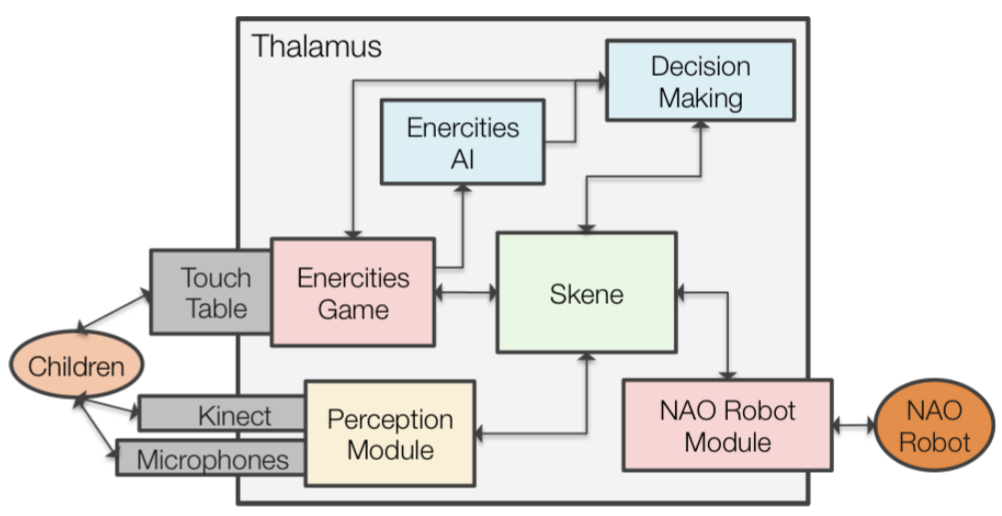
\includegraphics[width=0.6\linewidth]{images/SERA_ExSystemEC.png}
	\caption{Enercities scenario system architecture integrated with the SERA framework. From~\cite{Tullio2015}.}
	\label{fig:SERA:Examples}
\end{figure}

%Another example, using the Keepon robot~\cite{Kozima2009} (Figure~\ref{fig:robots:Keepon}) to keep ``early adolescents engaged in physical activity over long periods of time''~\cite{Tullio2015}.

\subsubsection*{Discussion}

Despite being under development, \ac{SERA} demonstrates its applicability in a wide range of \ac{HRI} scenarios. For example, the framework was used in the EMOTE project\footnote{\url{http://www.emote-project.eu}} with several publications on tutoring scenarios using different autonomous emphatic robots such as \ac{EMYS} (Figure~\ref{fig:robots:EMYS}) and NAO (Figure~\ref{fig:robots:NAO}). However, the \textit{Skene} component lacks dedicated rapport model and it does not adapt its actions when interrupted by the user, which reduces coordination and the overall feeling of rapport. Moreover, the \textit{Skene} component is rule-based which is not sufficiently elegant to build systems more appealing and natural to end-users.

\begin{figure}[H]
	\centering
	\begin{minipage}[b]{.4\textwidth}
		\centering
		\frame{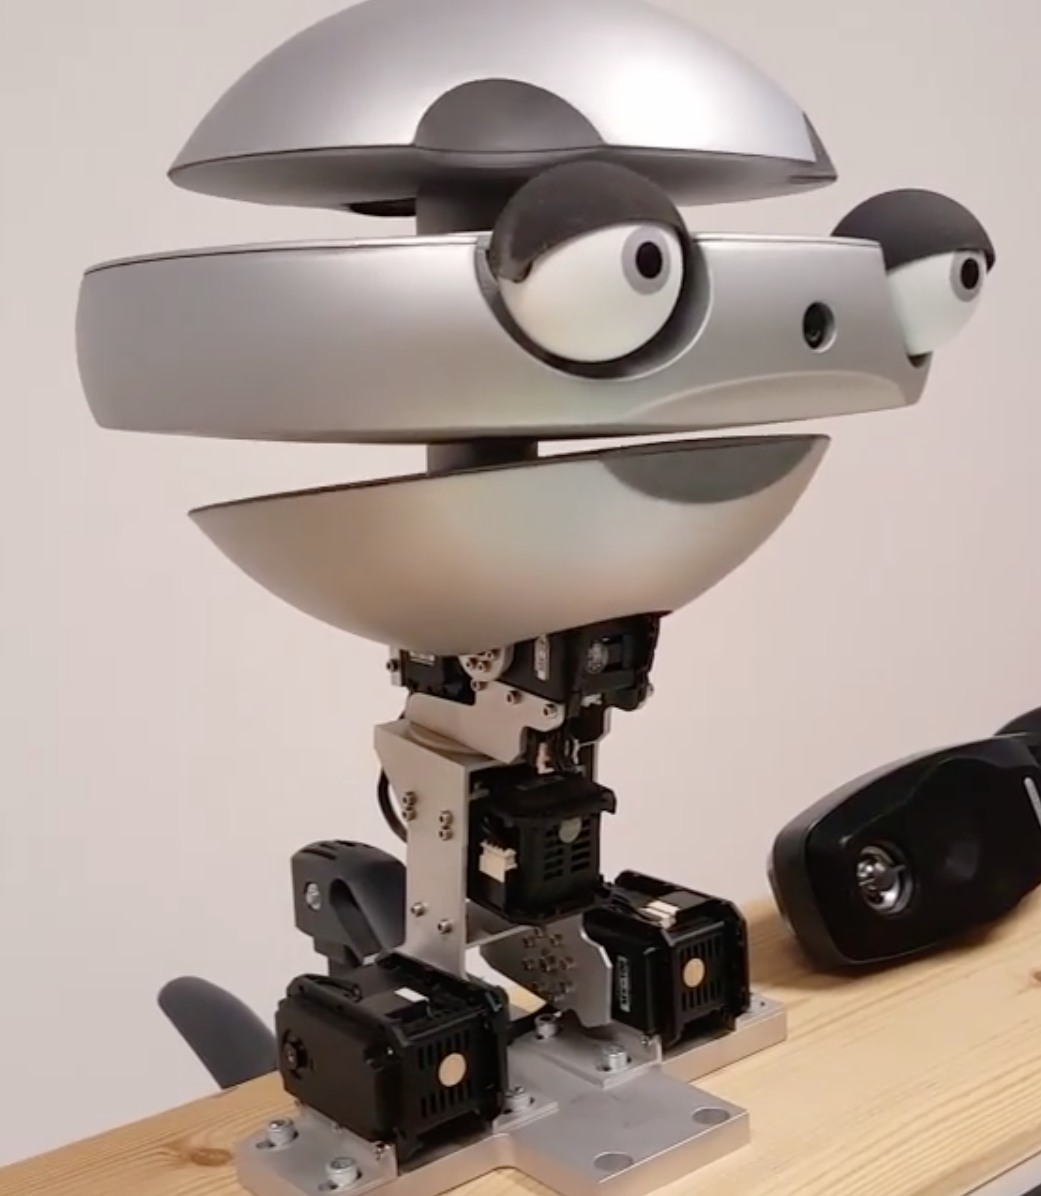
\includegraphics[width=0.4\textwidth]{images/emys.png}}
		\caption{EMYS robot.}
		\label{fig:robots:EMYS}
	\end{minipage}
%	\hfill
	\begin{minipage}[b]{.4\textwidth}
		\centering
		\frame{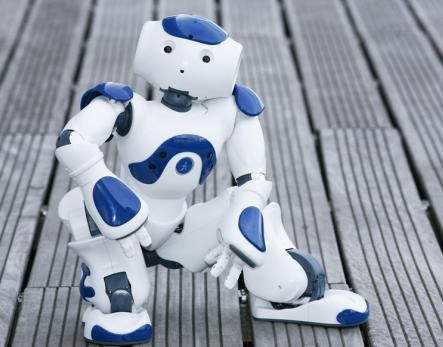
\includegraphics[width=0.55\textwidth]{images/NAO_Robot.JPG}}
		\caption{NAO robot.}
		\label{fig:robots:NAO}
	\end{minipage}
\end{figure}